%Deep Learning

%CNNs
Convolutional Neural Networks (CNNs) have become extremely popular and being used to solve a variety of image recognition problems. 
More recent and advanced CNN architectures have become deeper and more complex haing 10 to 20 
layers of Rectified Linear Units, hundreds of millions of weights, and billions of connections between units.
The reader is pointed to ~\cite{Bengio2009} for insights on deep architectures in general and ~\cite{DNNNature2015} for CNN-based learning and their recent advances.

While CNNs are an important thrust of research, they tend to be computationally expensive and deploying them on mobile platforms results in huge memory overheads. 
Another important insight recently unearthed by ~\cite{facenet}, is that the accuracies of CNNs can saturate after a few million images of training data.
Also the overall efficacy of the image recognition pipeline is contingent upon having a good region proposal scheme that feeds regions of interest (RoIs) into the CNN. 
A variety of strategies can be used to augment the capabilities of neural networks and we discuss a few below.

\subsection{Visual Attention}
Humans process only certain streams of visual information depending upon the task at hand. 
From a systems perspective, visual attention can be used as an efficient mechanism to prioritize visual processing.  
Pixel-level saliency models such as Attention by Information Maximiztion (AIM)~\cite{Bruceb} can be used in 
automatic household pantry organization and maintenance, particularly 
as part of visual assist systems for the visually impaired. Computationally, AIM determines visual salience based on the amount of information present in 
local regions of the image within the context of its surrounding region. 
Suppose a product (say cookies) is wrongly placed in a shelf that stores products of another type (say shampoo), the segment of the shelf image containing cookies is 
``less likely'' (higher self-information) to appear in the scene which mostly has image patches of shampoo, 
and therefore it is easily distinguishable or is considered ``salient''. This is shown in Figure~\ref{tab:saliencya}.
Once a salient region is detected, a second stage of object classification can be deployed to identify the wrongly placed object.  

%Saliency App 1
\begin{figure}[!htb]
\centering
\begin{tabular}{@{}l@{} @{}l@{}}
\vspace{-5pt}
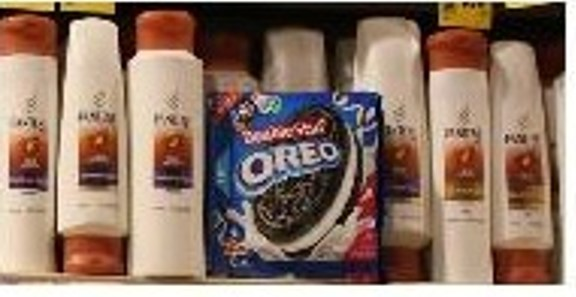
\includegraphics[width=0.5\linewidth,trim={0 0 0 0},clip]{mp1a.jpg} & 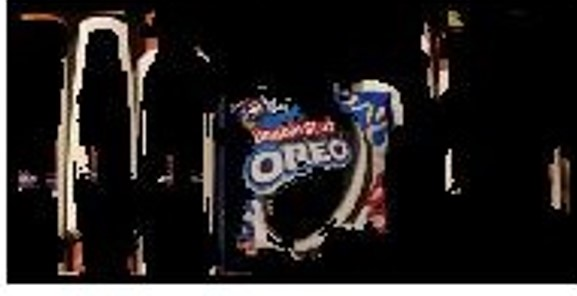
\includegraphics[width=0.5\linewidth,trim={0 0 0 0},clip]{mp1b.jpg}\\[\abovecaptionskip]
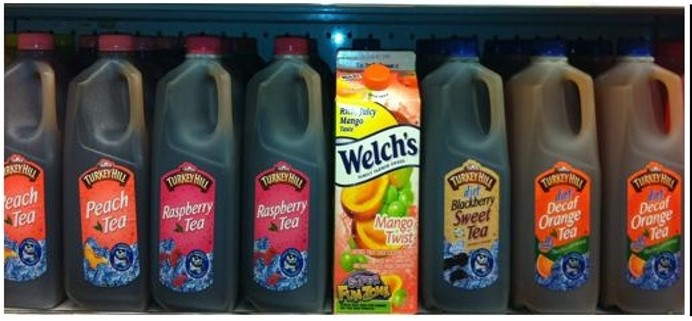
\includegraphics[width=0.5\linewidth,trim={0 0 0 0},clip]{mp2a.jpg} & 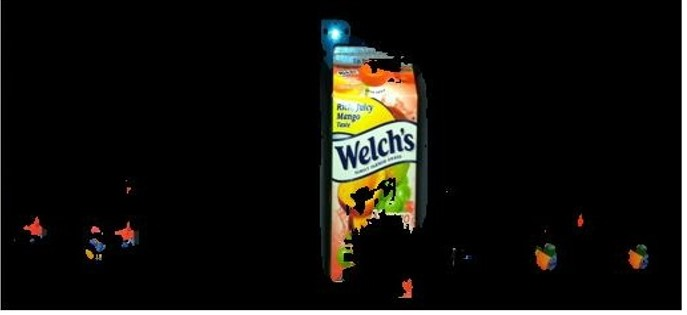
\includegraphics[width=0.5\linewidth,trim={0 0 0 0},clip]{mp2b.jpg}\\[\abovecaptionskip]
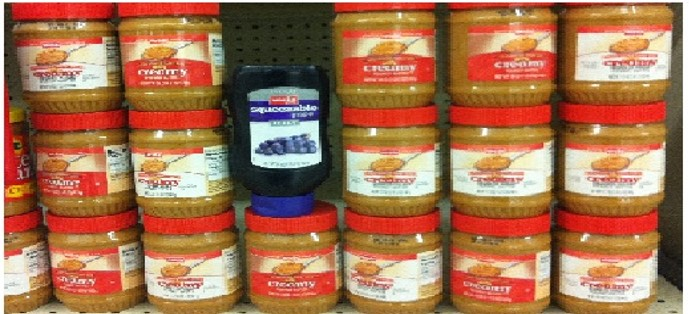
\includegraphics[width=0.5\linewidth,trim={0 0 0 0},clip]{mp3a.jpg} & 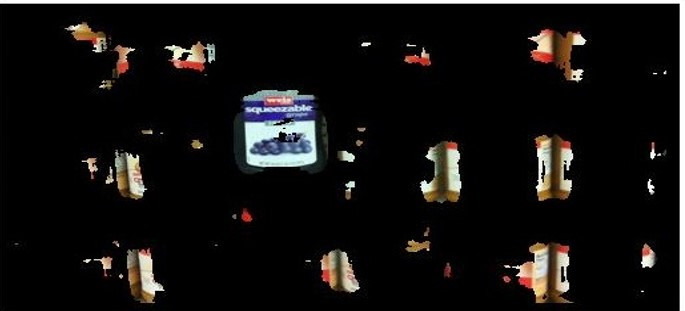
\includegraphics[width=0.5\linewidth,trim={0 0 0 0},clip]{mp3b.jpg}\\[\abovecaptionskip]
\small(a) Original image & \small (b) Thresholded saliency map\\
\end{tabular}
\caption{Saliency used for missplaced item detection.}
\label{tab:saliencya}
\end{figure}

\subsection{Redundancy}
A lot of visual scenes exhibit redundancy in some form or the other. 
For example, in a grocery aisle there are a lot of similar looking products like cereal boxes, detergent bottles, etc. Rather than processing each of these items 
as independent entities, we can localize similar RoIs, run our classification engine on only one of them and then assign the corresponding label to all of the similar 
RoIs. Figure~\ref{tab:saliencyb} illustrates this flow where AIM is used to generate initial seed RoIs that are then coupled with SURF keypoint matching 
to generate a list of RoIs that are similar in structure. 

%Saliency App 2
\begin{figure*}[!htb]
\centering
\begin{tabular}{@{}c@{} @{}c@{} @{}c@{}}
\vspace{-5pt}
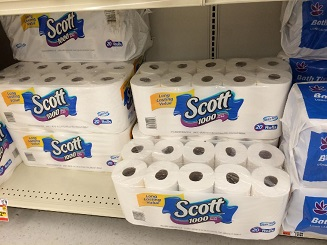
\includegraphics[width=0.32\linewidth,trim={0 0 0 0},clip]{scott_img.jpg} & 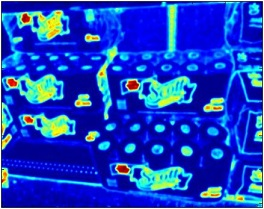
\includegraphics[width=0.31\linewidth,trim={0 0 0 0},clip]{scott_sali.jpg} & 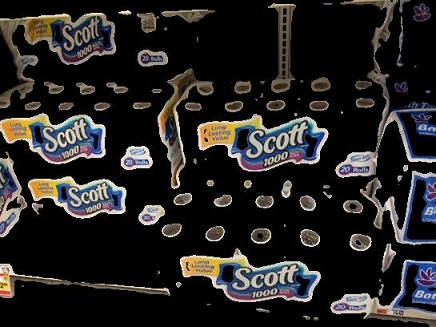
\includegraphics[width=0.32\linewidth,trim={0 0 0 0},clip]{scott_roi.jpg}\\[\abovecaptionskip]
\small(a) Original image & \small (b) Saliency Map & \small (c) Thresholded Map \\
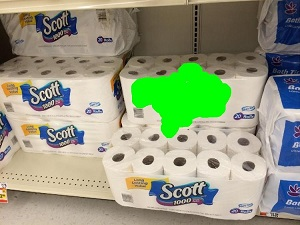
\includegraphics[width=0.32\linewidth,trim={0 0 0 0},clip]{scott_best_roi.jpg} & 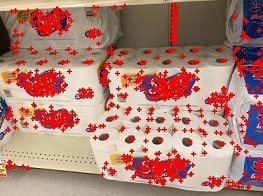
\includegraphics[width=0.32\linewidth,trim={0 0 0 0},clip]{scott_surf2.jpg} & 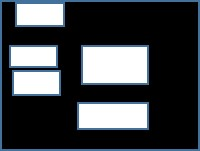
\includegraphics[width=0.32\linewidth,trim={0 0 0 0},clip]{scott_mask.jpg}\\[\abovecaptionskip]
\small(a) Best RoI & \small (b) SURF keypoints & \small (c) Regions of Interest \\
\end{tabular}
\caption{Saliency and SURF used to identify similar items.}
\label{tab:saliencyb}
\end{figure*}

\subsection{Context}
% Hierarchy of Parts
While deep learning models use learnt features to recognize objects in a scene, another contrasting approach is to use graphical models that build hierarchical 
representations of objects~\cite{hop}. Compositional rules can be used to build context cues to recognize objects never seen before. For example, an object having 
four wheels can be classified as a vehicle even if it is a new model of a car. 
% Spatial Context
While CNNs have been widely used for image category recognition, when it comes to recognizing objects in video streams, spatial context can play a huge role in 
reducing the workload on these computationally intensive classifiers. As shown in Figure~\ref{fig:viconet}, visual scenes can be represented as a knowledge graph.   
For example, in ~\cite{estimedia2015}, the authors proposed a Bayesian network called Visual Co-occurrence Network (ViCoNet) to not 
only improve the performance of their system, but also increase the recognition rates.

\begin{figure}[!htb]
\centering
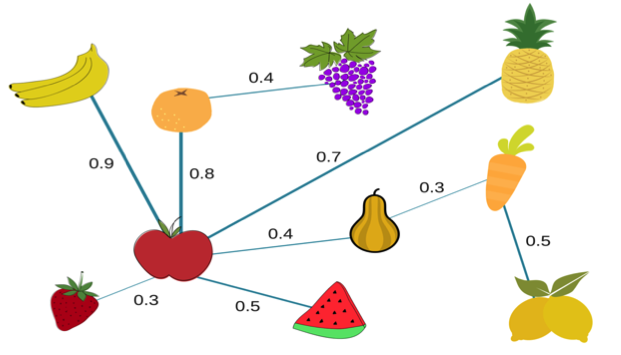
\includegraphics[width=0.9\linewidth]{viconetexample.png}
\caption{Spatial relations exist between frequently co-occurring objects. These relationships can then be used as context cues to guide the classifiers.}
\label{fig:viconet}
\end{figure} 

\subsection{Multimodal Fusion}
Humans use multisensory information from different sensory systems and combine it to influence 
perception, decisions, and overt behavior~\cite{stein2009neural}. Wearables can be used in a similar fashion to help users in different tasks. 
A rich topic of exploration is figuring out a way to fuse multi-sensor information, especially data from vision that is fundamentally two-dimensional with a temporal 
unidimensional stream of data from other sensors to make predictions of the current state of the user. Multi-sensor information coming in from different devices can be 
streamed to distributed networks that can then make real-time updates. In Figure~\ref{tab:sensor}, we illustrate data recorded from a wearable device while two users
walk in three different directions. These sensors are sensitive enough to be used as localization cues. 

%MultiModal Analysis
\begin{figure}[!htb]
\centering
\begin{tabular}{@{}c@{} @{}c@{}}
\vspace{-5pt}
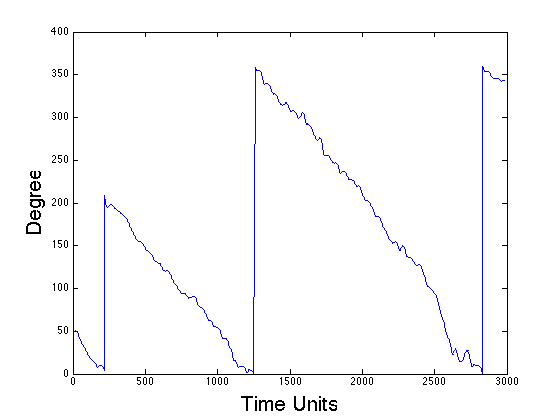
\includegraphics[width=0.5\linewidth,trim={0 0 0 0},clip]{walk_left_p1.png} & 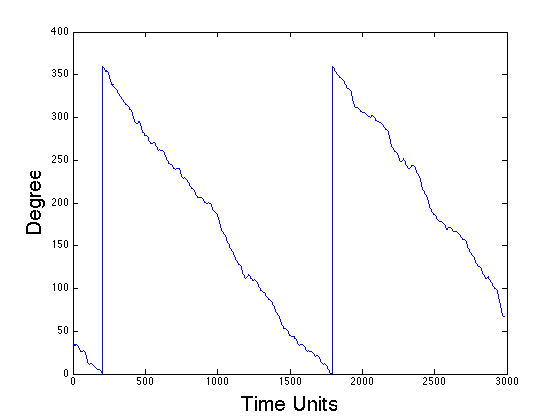
\includegraphics[width=0.5\linewidth,trim={0 0 0 0},clip]{walk_left_p2.png}\\[\abovecaptionskip]
\small(a) Person 1 - Left & \small (b) Person 2 - Left\\
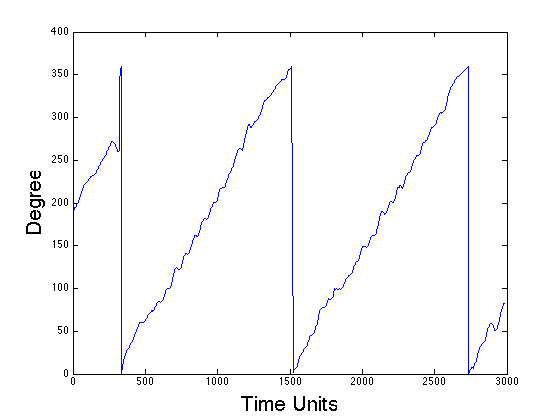
\includegraphics[width=0.5\linewidth,trim={0 0 0 0},clip]{walk_right_p1.png} & 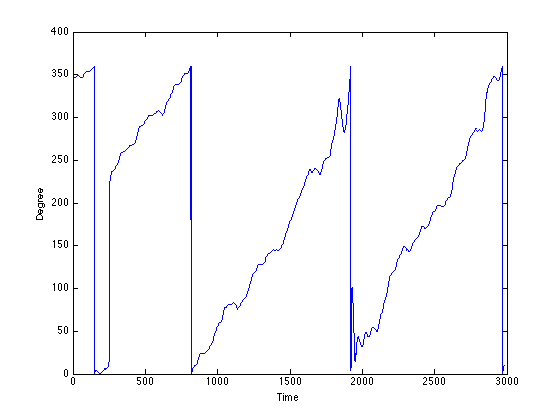
\includegraphics[width=0.5\linewidth,trim={0 0 0 0},clip]{walk_right_p2.png}\\[\abovecaptionskip]
\small(a) Person 1 - Right & \small (b) Person 2 - Right\\
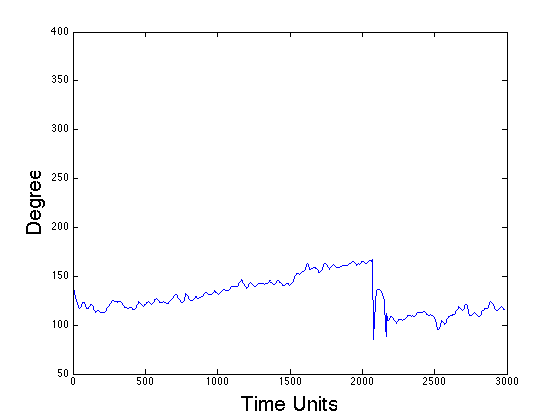
\includegraphics[width=0.5\linewidth,trim={0 0 0 0},clip]{walk_straight_p1.png} & 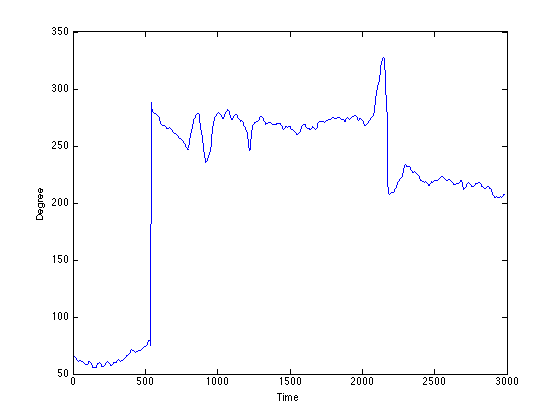
\includegraphics[width=0.5\linewidth,trim={0 0 0 0},clip]{walk_straight_p2.png}\\[\abovecaptionskip]
\small(a) Person 1 - Straight & \small (b) Person 2 - Straight\\
\end{tabular}
\caption{Other sensor information used for localization.}
\label{tab:sensor}
\end{figure}
